\documentclass[a4paper, 11pt]{article}
\usepackage{geometry}
\geometry{letterpaper, margin=1in}
\usepackage{graphicx}
\graphicspath{ {images/} }

\usepackage{amsmath}
\usepackage{amssymb}  
\usepackage{amsthm}
\usepackage{ulem}

\usepackage{enumitem}


\usepackage{pdfpages} % for including full pdf pages

% format to allow bolded theorems, corollaries, etc... 
\newtheorem*{theorem}{Theorem}
\newtheorem*{corollary}{Corollary}
\newtheorem*{lemma}{Lemma}
\newtheorem*{definition}{Definition}
\newtheorem*{Example}{Example} 
\newtheorem*{Remark}{Remark}

% stop typing \mathbb a thousand times 
\newcommand{\R}{\mathbb{R}}
\newcommand{\C}{\mathbb{C}}
\newcommand{\F}{\mathbb{F}}

% commands for bra-ket notation
\newcommand{\bra}[1]{\ensuremath{\left\langle#1\right|}}
\newcommand{\ket}[1]{\ensuremath{\left|#1\right\rangle}}
\newcommand{\bracket}[2]{\ensuremath{\left\langle #1 \middle| #2 \right\rangle}}
\newcommand{\matrixel}[3]{\ensuremath{\left\langle #1 \middle| #2 \middle| #3 \right\rangle}}
\newcommand{\expectation}[1]{\ensuremath{\left\langle #1 \right\rangle}}

% change margins for solution
\newenvironment{solution}{%
	\begin{list}{}{%
			\setlength{\topsep}{0pt}%
			\setlength{\leftmargin}{0.5cm}%
			\setlength{\rightmargin}{0.5cm}%
			\setlength{\listparindent}{\parindent}%
			\setlength{\itemindent}{\parindent}%
			\setlength{\parsep}{\parskip}%
		}%
		\item[]}{\end{list}}



\begin{document}
\noindent
\large\textbf{PH 424} \hfill \textbf{Separation of
  Variables: The diffusion equation} \\
 \hfill  Date: \today \\
\par\noindent\rule{\textwidth}{0.4pt} \\\\


\noindent Consider the temperature of a one-dimensional metal rod of length L
given by the function $u(x,t)$. The temperature of this rod is given by the one
dimensional diffusion equation
\begin{equation}
  \frac{1}{\alpha}\frac{\partial u}{\partial t} = \frac{\partial^2 u}{\partial x^2}
\end{equation}

\noindent If both ends of the metal rod are \textit{insulated}, then the temperature will
obey the following boundary conditions.  Why?
\begin{align}
  \left. \frac{\partial u(x,t)}{\partial{x}} \right\vert_{x=0} &= 0 \\
  \left. \frac{\partial u(x,t)}{\partial{x}} \right\vert_{x=L} &= 0
\end{align}
This can be written more compactly as
\begin{align}
  u'(0,t) &= 0  \\
  u'(L, t) &= 0 
\end{align}

\begin{enumerate}[leftmargin=0em]
  \item \textbf{Use separation of variables to find an analytical solution for
      $u(x,t)$. Specify how you chose or identified your separation constants.}\\
    \begin{solution}
      The separation of variables procedure for partial differential equations
      (PDEs) begins by making the clever ansatz.
      \begin{equation}
        \textbf{ANSATZ:}\quad u(x,t) = X(x)T(t)
      \end{equation}
     which says that the dependence of the temperature $u(x,t)$ on the independent
     variables can be written as the product of a function that depends only
     on x with a function that depends only t.  If we plug this back into
     equation (1) we find that our ansatz significantly simplifies the
     differential equation.
     \begin{align}
       \frac{1}{\alpha}\frac{\partial}{\partial t}\;X\;T &= \frac{\partial^2}{\partial x^2}\;X\;T \\
       \frac{1}{\alpha}\left( \frac{\partial T}{\partial t} \right) X &= \left( \frac{\partial^2 X}{\partial x^2} \right) T
     \end{align}
    Notice how the partial derivatives only apply to the function of the
    corresponding independent variable. Now we can divide both sides by
    $X(x)T(t)$ so that the equation becomes 
    \begin{equation}
      \frac{1}{\alpha \; T}\left( \frac{\partial T}{\partial t} \right) = \frac{1}{X}\left( \frac{\partial^2 X}{\partial x^2} \right)
    \end{equation}
    At this point we can see that all of the $t$ dependence is on the left hand
    side of the equation and all of $x$ dependence is on the right. Furthermore,
    because $X(x)$ and $T(t)$ are equations of only one variable, what were
    partial derivatives ($\partial/\partial t$, $\partial^2 / \partial x^2$) are
    now ordinary derivatives ($d/dt$, $d^2/dx^2$). \\

    \noindent In summary, we have reformulated the PDE as
    \begin{equation}
      \frac{1}{\alpha \; T(t)}\frac{d T(t)}{dt} = \frac{1}{X(x)}\frac{d^2 X(x)}{dx^2}
    \end{equation}
    
    Now comes the ``\textit{say some magic}'' part Corinne talked about in class.
    Imagine we fix $x$ to be some value. Then, the right hand side of equation
    (10) is  constant. If we then allow $t$ to vary, the function $T(t)$ will
    certainly change, but the combination of $T$ with its derivative on the
    L.H.S. must remain constant because we know that the R.H.S. is constant. Let's call this constant $A$.
    Then we have
    \begin{align}
      \frac{1}{\alpha\; T(t)}\frac{d T(t)}{dt} &= A \\
      \frac{1}{X(x)}\frac{d^2 X(x)}{dx^2} &= A
    \end{align}

    Some rearranging gives
    \begin{align}
      \frac{d T(t)}{dt} &= \alpha A\; T(t) \\
      \frac{d^2 X(x)}{dx^2} &= A\;X(x)
    \end{align}
    
    We have turned a partial differential equation into two homogeneous ordinary
    differential equations with constant coefficients! 
		
		Recall that our boundary
    conditions were given with respect to $x$. Therefore, we will solve equation
    (14) before we solve the tempting first-order time equation.

    \begin{align}
      \textbf{ANSATZ:} \quad &X(x)= e^{rx} \\
      \text{plug into 14:}\quad &\frac{d^2}{dx^2}e^{rx} - Ae^{rx}= 0 \\
      &(r^2-A)e^{rx}= 0 \\
      &r^2-A= 0 \\
      &r= \pm\sqrt{A} \\
      \Rightarrow &X(x)= c_+e^{\sqrt{A}x}+c_-e^{-\sqrt{A}x}
    \end{align}
    Now that we have found a functional form for $X(x)$ we can apply our boundary
    conditions. 
    \begin{align}
      u'(0,t) = X'(0)T(t) = 0 \\
      u'(L,t) = X'(L)T(t) = 0 
    \end{align}
    These boundary conditions need to be true for all values of $t$, therefore:
    \begin{align}
      X'(0) &= 0 \\
      X'(L) &= L 
    \end{align}
    
    Applying (23) to (20) gives
    \begin{align}
      X'(x) &= \sqrt{A}c_+e^{\sqrt{A}x}-\sqrt{A}c_-e^{-\sqrt{A}x} \\
      X'(0) &= \sqrt{A}c_+-\sqrt{A}c_- \\
      \Rightarrow c_+-c_- &= 0 \\
      c_+ &= c_- \\
      \Rightarrow X(x) &= c_+e^{\sqrt{A}x}+C_+e^{\sqrt{A}x}
    \end{align}
    
    In class we tried to use this solution to match the boundary condition for
    the case where $A>0$. This is impossible as the derivative becomes a $\sinh$
    function that only takes the value 0 at the origin. What happens if we let
    the constant be $A<0$?

    \begin{align}
      X(x) &= c_+e^{-i\sqrt{|A|}x}+c_+e^{i\sqrt{|A|}x} \\
       &= c_+\cos(\sqrt{A}x) 
    \end{align}
   Where in the last step I have identified the combination of complex
   exponentials in (30) as a cosine and absorbed the extra factor of 2 into the
   constant $c_+$. Now we can try to apply the second boundary condition (24).
   \begin{align}
     X'(L) &= -\sqrt{|A|}c_+\sin(\sqrt{|A|}L) = 0 \\
     \sin(\sqrt{|A|}L) &= 0 \\
     \Rightarrow \sqrt{|A|}L &= n\pi \\
     |A| &= \frac{n^2 \pi^2}{L^2}\\
		 A &= -\frac{n^2 \pi^2}{L^2}
   \end{align}
   As $\cos(-\theta)=\cos(\theta)$ negative values of n are redundant so that
   $n = 0, 1, 2, 3, ...$ We have found that
   \begin{align}
     X(x) &= c_+\cos\left(\frac{n\pi x}{L}\right)\\
     A &= -\frac{n^2\pi^2}{L^2}
   \end{align}
   Now that we know $A$, we can solve the time equation (13). It is
   \begin{equation}
     \frac{d}{dt}T(t) = -\frac{\alpha \pi^2 n^2}{L^2}T(t)
   \end{equation}

   We an use the same ansatz to solve this differential equation.
   \begin{align}
     \textbf{ANSATZ:}\quad T(t) &= e^{st} \\
     \frac{d}{dt}e^{st}+\frac{\alpha\pi^2n^2}{L^2}e^{st}&= 0 \\
     \left( s+\frac{\alpha \pi^2n^2}{L^2} \right)e^{st}&=0  \\
     s &= -\frac{\alpha \pi^2 n^2}{L^2} \\
     \Rightarrow T(t) &= d\; e^{-\frac{\alpha \pi^2}{L^2}t} 
   \end{align}

   Where d is a constant to be determined by the initial conditions. \\

   Let's pause and reflect on what we have found so far. After performing the
   separation of variables procedure on the diffusion equation we found that it
   reduced to two ordinary, homogeneous differential equations with constant
   coefficients. Each of these differential equations is independently equal to
   some constant $A$. \\

   We chose to solve the second ODE (eqn 14) first because our boundary conditions
   are given in terms of $x$. At this point, $A$ was still a free parameter.
   Solving this ODE with the boundary conditions determined the value of $A$. Knowing this
   constant, we then solved the equation for $T(t)$. We can now write the full
   solution as

   \begin{equation}
     u(x,t) = X(x)T(t) = \beta\cos\left(\frac{n\pi x}{L}\right)e^{-\frac{\alpha n^2\pi^2}{L^2}t}
   \end{equation}
   
   Note that I have combined the constants $d$ and $c_+$ into one constant
   called $\beta$. Now we are almost done. We know everything in the equation for
   $u(x,t)$ except for the constant $\beta$. It must be determined by the initial
   conditions. \\

   Before we move on though, we have one more observation to make. Both of the
   derivative operators in the diffusion equation (1) are linear because
   differentiation is linear. This means
   that if we take a linear combination of solutions for different values of $n$,
   the diffusion equation will still be satisfied. Therefore the most general
   way we can write the temperature function would be to include a term for each
   possible value of $n$.
   \begin{equation}
     u(x,t) = \sum\limits_{n=0}^{\infty} \beta_n\cos\left(\frac{n\pi x}{L}\right)e^{-\frac{\alpha n^2\pi^2}{L^2}t}
   \end{equation}

   The fact that we have this combination of terms means that we can now write
   $u(x,t)$ to match any reasonably well behaved initial conditions as we will
   see in the next part of the problem. 
    
    \end{solution}

    \item \textbf{Suppose you know the initial temperature of the rod has the
        functional form $u(x,0)=300+28\cos^3\left(\frac{\pi x}{L}\right)$
        Kelvin. Find a closed form solution for the temperature $u(x,t)$ for all
        $t>0$. Do some sense-making about your solution.}\\
      
      \begin{solution}
        First let's graph this initial temperature distribution to see what it
        looks like.
        \begin{figure}[!hbt]
          \centering
          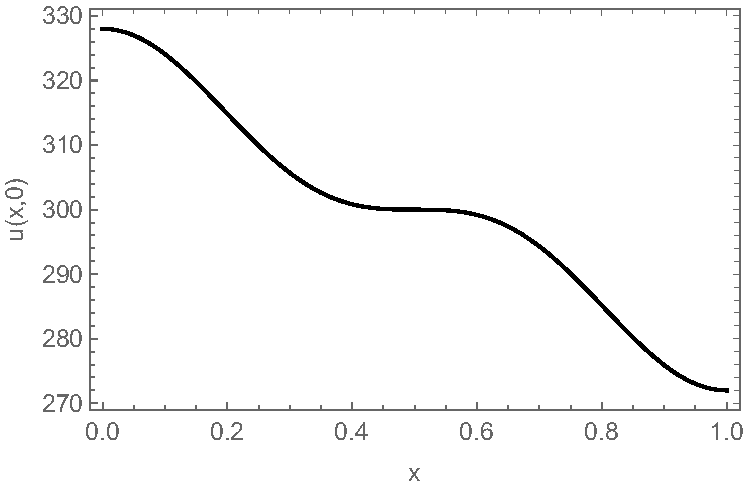
\includegraphics[width=.75\columnwidth]{initial_configuration}
          \caption{The initial temperature configuration of the system with
            $L=1$}
          \label{fig:initial_configuration}
        \end{figure}
				
        Setting $t=0$ in (45) gives us
        \begin{equation}
          u(x,0) = \sum\limits_{n=0}^\infty \beta_n\cos\left(\frac{n\pi x}{L}\right)
        \end{equation}
        To be able to expand (46) to match (45), we want an
        orthogonality relationship between the cosine terms.  We will make a guess based on our
				experience from Fourier series and check:
        \begin{align}
          \int\limits_0^L \cos\left(\frac{n\pi x}{L}\right)\cos\left(\frac{m\pi x}{L}\right)dx &= \frac{1}{4}\int\limits_0^L \left( e^{in\pi x/L}+e^{-in\pi x/L} \right)\left( e^{im\pi x/L}+e^{-im\pi x/L} \right)dx \\
              &= \frac{1}{4}\int\limits_0^L e^{i(n+m)\pi x/L}+e^{-i(n+m)\pi x/L}\\
              &\hspace{5em}+e^{i(n-m)\pi x/L}+e^{-i(n-m)\pi x/L}dx \\
              &= \frac{1}{2}\int\limits_0^L\Big\{ \cos\big((n+m)\pi x/L \big) +\cos\big( (n-m)\pi x/L \big) \Big\}dx
        \end{align}
        \begin{align}
          &= \left.\frac{1}{2}\Big\{ \frac{L}{(n+m)\pi}\sin\Big((n+m)\pi x/L\Big) + \frac{L}{(n+m)\pi}\sin\Big((n-m)\pi x/L\Big)\Big\}\right\vert_0^L \\
          &= \frac{1}{2}\Big\{ \frac{L}{(n+m)\pi}\sin\Big((n+m)\pi\Big) + \frac{L}{(n+m)\pi}\sin\Big((n-m)\pi\Big)\Big\} 
        \end{align}
        Now we have two cases to explore. The first is for $n\neq m$. Since
        $n,m$ are both integers, then certainly $n+m$ and $n-m$ are both
        integers and therefore
        \begin{align}
          \sin\big((n+m)\pi\big)=\sin\big((n-m)\pi\big) &= 0  \\
          \Rightarrow \int_0^L \cos(n\pi x/L)\cos(m\pi x/L)dx &= 0 
        \end{align}
        If $n=m$, then the first term in (53) is zero but the second term
        becomes $\frac{0}{0}$. If we use L'Hopital's rule to evaluate, then the
        equation becomes
        \begin{align}
          \int\limits_0^L \cos^2(n\pi x/L)dx &= \lim\limits_{(n-m)\to 0}\;\;\frac{1}{2}\frac{L}{(n+m)\pi}\sin\big( (n-m)\pi  \big) \\
                                             &= \frac{L}{2}\lim\limits_{(n-m)\to 0}\;\; \frac{\frac{d}{d(n-m)}\sin\big( (n-m)\pi \big)}{\frac{d}{d(n-m)}(n-m)\pi} \\
                                             &= \frac{L}{2}\lim\limits_{(n-m)\to 0}\frac{\pi\cos\big((n-m)\pi\big)}{\pi} \\
          &= \frac{L}{2} 
        \end{align}

        Lastly, because $n=0$ is also a valid choice, we have an exception to
        (59) given by
        \begin{align}
          \int\limits_0^L \cos^2(0)dx &= \int\limits_0^L dx = L
        \end{align}
        
        Thus, we conclude that
        \begin{equation}
          \int\limits_0^L \cos(n\pi x/L)\cos(m\pi x/L)dx =  
          \begin{cases}
            \frac{L}{2}\delta_{m,n} &\text{for } n,m\neq 0\vspace{1em}\\
            L &\text{for } n=m=0
          \end{cases}
        \end{equation}
        and therefore the cosines are orthogonal. In recognition of this oddity
        for $n=0$, let's rewrite (47) in anticipation of the expansion we want
        to perform for $u(x,0)$.
        \begin{equation}
          u(x,0) = \frac{\beta_0}{2} +\sum\limits_{n=1}^\infty\beta_n \cos\left( \frac{n\pi}{L}x \right)
        \end{equation}

        Our goal now is to solve for the $\beta_n$ coefficients in the
        expansion of our initial condition. We know how combinations
        of cosines behave under the integration rule (61) so we can solve for
        $\beta_n$'s using what's called \textit{Fourier's trick}. First multiply
        both sides of (62) by an arbitrary cosine term and then integrate over
        the rod.  
        \begin{align}
          u(x,0)\cos\left( \frac{m\pi}{L}x \right) &= \Bigg[ \frac{\beta_0}{2} +\sum\limits_{n=1}^\infty\beta_n \cos\left( \frac{n\pi}{L}x \right)\Bigg]\cos\left( \frac{m\pi}{L}x \right)\\
          \int_0^Lu(x,0)\cos\left( \frac{m \pi}{L}x \right) &= \int_0^L\frac{\beta_0}{2}\cos\left( \frac{m\pi}{L}x \right)dx\\
                                                   &\hspace{2em}+ \int_0^L\sum\limits_{n=1}^\infty \beta_n\cos\left(\frac{n\pi}{L}x \right)\cos\left( \frac{m\pi}{L}x \right)dx \\
                                                   &= \frac{\beta_0}{2}\int_0^L\cos\left( \frac{0\pi}{L}x \right)\cos\left( \frac{m\pi}{L}x \right)dx \\
                                                   &\hspace{2em}+\sum\limits_{n=1}^\infty\beta_n\int_0^L\cos\left( \frac{n\pi}{L}x \right)\cos\left( \frac{m\pi}{L}x \right)dx  \\
                                                   &= \frac{\beta_0}{2}L\delta_{0,m}+\sum\limits_{n=1}^\infty\beta_n\frac{L}{2}\delta_{n,m} \\
                                                   &= \frac{L}{2}\sum\limits_{n=0}^\infty \beta_n\delta_{n,m} = \frac{L}{2}\beta_m 
        \end{align}
        \begin{equation}
        \Rightarrow\boxed{\beta_m = \frac{2}{L}\int_0^Lu(x,0)\cos\left( \frac{m\pi}{L}x \right)dx} 
        \end{equation}
        

        
        At this point, we could solve the integral in (70) in order to
        determine the coefficients for the expansion in (62). In some cases, it
        is more convenient to try and manipulate the initial condition so that the
        coefficients can be identified by inspection. For us this amounts to
        using some trigonometry to rewrite the cosine cubed term.
        \begin{align}
          \text{recall: }\quad \cos^3(\beta)&= \frac{1}{4}\Big(3\cos(\beta)+\cos(3\beta)\Big) \\
          \Rightarrow u(x,0)&= 300+21\cos\left(\frac{\pi x}{L}\right)+7\cos\left( \frac{3\pi x}{L} \right)\\
          \Rightarrow &\begin{cases}
            \beta_0 = 600 \\
            \beta_1 = 21 \\
            \beta_3 = 7
            \end{cases}
        \end{align}
        Therefore, the closed form solution for the temperature given the
        initial conditions is
        \begin{equation}
          u(x,t)= 300+21\cos\left( \frac{\pi x}{L} \right)e^{-\frac{\alpha\pi^2}{L^2}t}+7\cos\left( \frac{3 \pi x}{L} \right)e^{-\frac{\alpha 9\pi^2}{L^2}t}
        \end{equation}

        ...and there we have it! Let's end with a little sense making. At $t=0$
        we have a temperature distribution along the rod that matches the
        initial conditions shown in figure \ref{fig:initial_configuration}. The
        time dependence is a decaying exponential. This matches our physical
        intuition because we know that without a source or sink for heat
        transfer to the rod, we expect the temperature should decay to some
        equilibrium value after a period of time.
      \end{solution}

      \item \textbf{Plot your solution in Mathematica for several different for
          several different instants in time including t=0. }\\
        \begin{solution}
          Figure \ref{fig:time_evolution} shows the temperature distribution at
          several different points in time. \\ 
          \begin{figure}[!hbt]
            \centering
            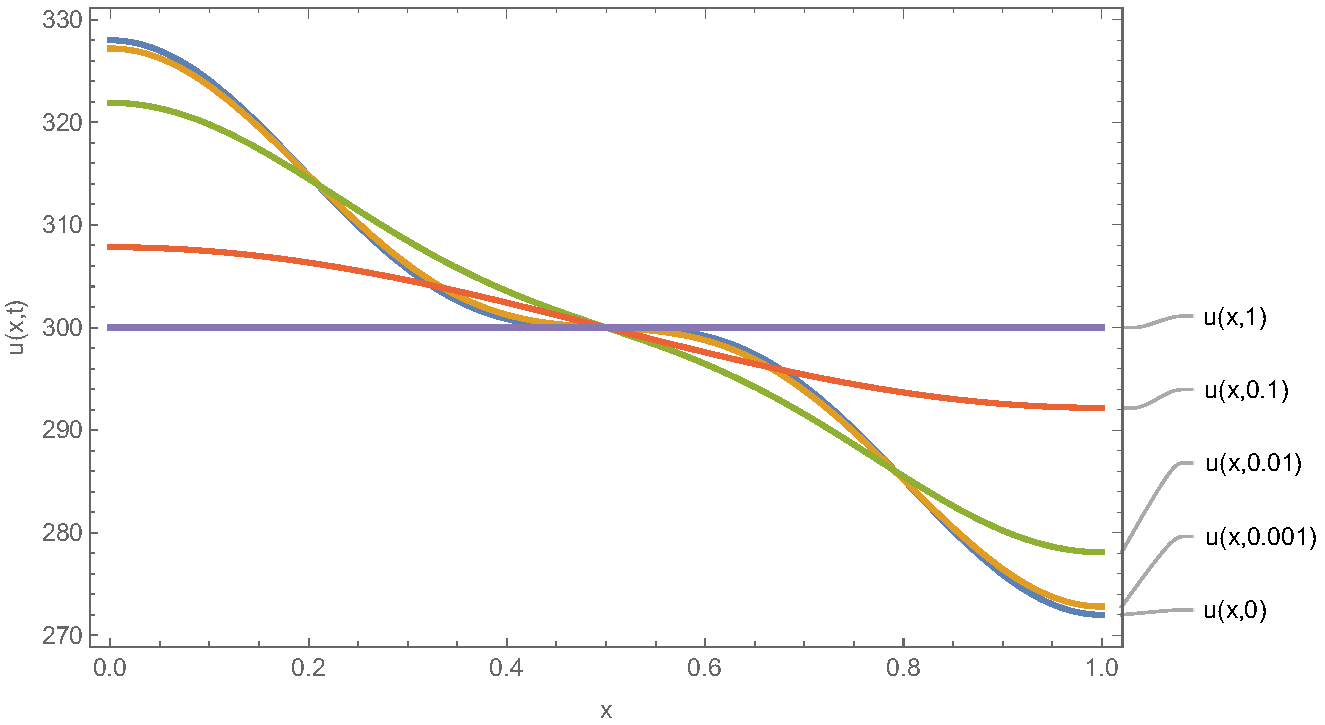
\includegraphics[width=1\columnwidth]{time_evolution}
            \caption{Graphs of the temperature distribution along the rod shown
              at various times starting at $t=0$. For this graph, I set
              $\alpha=1$, and $L=1$}
            \label{fig:time_evolution}
          \end{figure}

          This does exactly what we said we expect after looking at equation
          (70)! The distribution tends towards an equilibrium value. Of course,
          the speed at which this occurs depends highly on the value of
          $\alpha$. Because $\alpha=1$ for this graph, the decay is very quick.
        \end{solution}
        
      
\end{enumerate}


\end{document}

































